\chapter{Architecture}
The MoVEAS project can be split into two major components: the client-side part, collecting and filter sensors' data, and the server-side one, receiving and manage that data.

\section{Client-side}
The data collected from the Photon basically flowed like as shown in the following schema:

\begin{center}
	\begin{figure}[ht]
		\makebox[\textwidth]{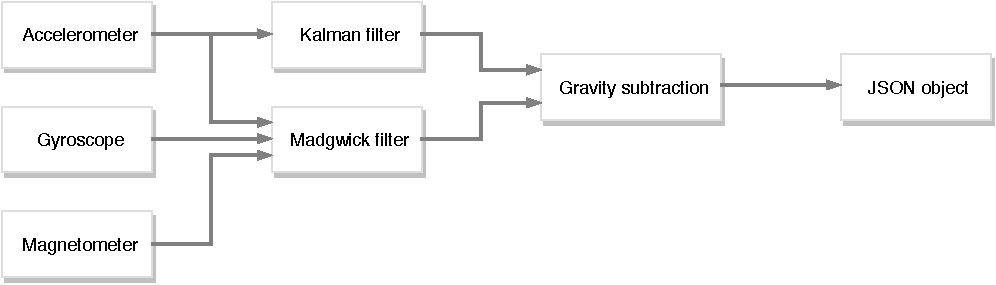
\includegraphics[width=0.65\paperwidth]{img/data_fusion_old.pdf}}
		\caption{Previous project's data fusion schema.} \label{old data fusion schema}
	\end{figure}
\end{center}
\bigbreak

As shown in the chapter \ref{Madgwick filter}, the Madgwick filter does not need Kalman filtered data\dots

\section{Server-side}
\dots
